\documentclass{article}

\PassOptionsToPackage{numbers,sort&compress}{natbib}
\usepackage[preprint]{neurips_2025}
\usepackage{newtxtext}

\usepackage{graphicx}
\usepackage{booktabs}
\usepackage{caption}
\usepackage{float}
\usepackage{xcolor}
\usepackage{hyperref}
\usepackage{enumitem}
\usepackage{array}
\usepackage{amsmath}

\hypersetup{colorlinks=true, linkcolor=black, urlcolor=blue!55!black, citecolor=black}
\setlist[itemize]{leftmargin=1.2em, itemsep=0.15em, topsep=0.15em}
\captionsetup{font=small, labelfont=bf}
\newcolumntype{L}[1]{>{\raggedright\arraybackslash}p{#1}}
\raggedbottom

\newcommand{\actmap}{\textit{ActMap}}
\newcommand{\ci}{\ensuremath{\pm}}

\title{ActMap: Activation Maps for LLM White-Box Uncertainty Quantification}
\author{%
  Jacopo Dardini \\
  Alma Mater Studiorum -- University of Bologna \\
  \texttt{jacopo.dardini@studio.unibo.it} \quad \texttt{0001169321}
}

\begin{document}
\maketitle

\begin{abstract}
Large language models can answer factual and reasoning questions fluently while being wrong, and scalar confidence scores make that failure hard to inspect. This report studies \actmap{}, a novel white-box uncertainty method that treats hidden-state trajectories as evidence rather than discardable byproducts of generation. The method converts runtime activations into a fixed activation map, then learns whether that map resembles trajectories that usually lead to correct or incorrect answers. Its goal is both ranking performance and an auditable intermediate artifact: a structured per-answer record that can support inspection, calibration monitoring, abstention, routing, and human oversight. Across TriviaQA, NQ-Open, WebQuestions, and GSM8K, \actmap{} is the strongest in-domain ranker against supervised white-box probes and black-box confidence scores. Because the score is tied to a tensor artifact rather than only to text or probabilities, it also gives a mechanistic interpretability handle for accountable deployment: systems can log the internal uncertainty signal, audit distribution shift, and route risky answers to review instead of presenting fluent errors without traceable evidence.
\end{abstract}

\begin{figure}[H]
    \centering
    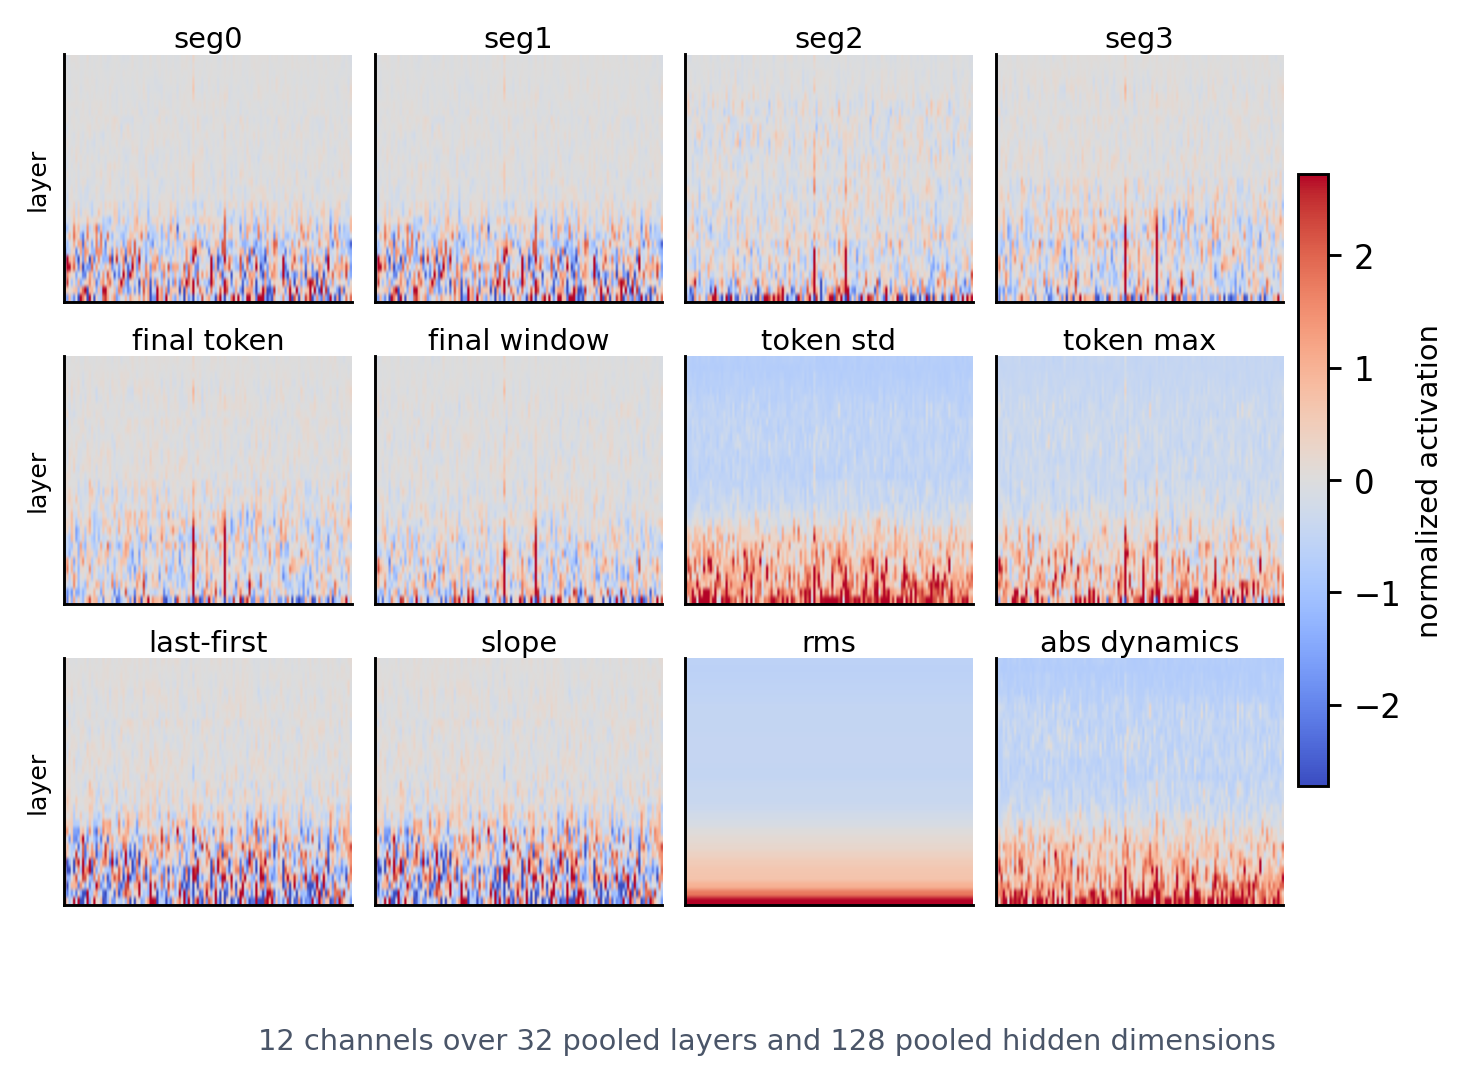
\includegraphics[width=0.78\linewidth]{figures/actmap_first_page.png}
    \caption{Twelve-channel \actmap{} view of a single generation. Each panel is one normalized channel over 32 pooled layers and 128 pooled hidden-dimension bins.}
    \label{fig:first-page-actmap}
\end{figure}

\section{Introduction}

This work was partly inspired by Anthropic's Natural Language Autoencoder (NLA) article~\cite{nla2026}, which treats activations as objects that can be compressed into a human-legible intermediate representation. \actmap{} pursues answer-level uncertainty instead: from the hidden-state trajectory collected \emph{during} generation, predict whether the model's answer is likely correct, while still treating internal states as inspectable evidence.

The motivation is both technical and ethical. Language models can produce concise, fluent, and false answers. In high-stakes or user-facing settings, this creates risks of overreliance, automation bias, and untraceable failure modes~\cite{weidinger2021}. Trustworthy AI guidance emphasizes robustness, transparency, human oversight, and accountability~\cite{hleg2019,nist2023}. A calibrated uncertainty signal can support those goals by routing risky outputs to retrieval, a stronger model, or a human reviewer.

Black-box confidence signals rely on generated text or token probabilities. They are easy to deploy, but they ignore most of the computation that produced the answer. Recent confidence-elicitation and factual-confidence studies show that these signals are useful but unstable, and that trained hidden-state probes can be stronger when model internals are available~\cite{mahaut2024,xiong2024}. White-box methods use hidden states and can access richer evidence. \actmap{} tests whether the full generation-time activation trajectory contains correctness information that is not captured by a single hidden state or a scalar token-likelihood statistic.

The core intuition is that \actmap{} reframes uncertainty detection as a spatial pattern-recognition problem. Instead of relying on one hidden vector, one layer, or one scalar confidence score, \actmap{} examines how activation energy is distributed across layers and token positions. Prior work makes this plausible from two directions: truthfulness and answer correctness can be decoded from hidden states~\cite{azaria2023,kadavath2022,marks2023,bhatnagar2026}, while semantic-entropy and explanation-stability methods show that unsupported answers spread across a higher-variance set of sampled meanings or rationales~\cite{becker2024,farquhar2024}. \actmap{} tests whether a similar stability gap leaves a measurable footprint in the generation trajectory itself. The classifier learns recurring activation geometry associated with reliable and fragile internal states. Five reasons explain why this can work:
\begin{itemize}
    \item \textbf{Correctness has semantic and computational signatures.} Even when the final text looks plausible, the model's internal computation can differ between supported recall or reasoning and guesswork.
    \item \textbf{Uncertainty is distributed.} A single layer or token can miss the signal, but a layer-by-token map can capture where uncertainty emerges, persists, or resolves.
    \item \textbf{The probe has the right inductive bias.} A classifier that attends jointly across layer-depth and temporal-channel axes captures distributed failure patterns that a single-vector readout would miss.
    \item \textbf{It is model-output agnostic at inference time.} Once the classifier is trained, \actmap{} needs no calibrated probabilities, verbalized confidence, or multiple sampled answers, so it stays usable when black-box heuristics are weak or answer formats change.
    \item \textbf{The signal is partly mechanistic.} Strong in-domain results on GSM8K argue against a detector that only memorizes QA lexical style, while the transfer gaps show the reliability geometry depends on task family and source coverage.
\end{itemize}

The main contribution is \actmap{}: a fixed-shape activation-map representation of generation-time hidden states paired with a ViT2D classifier for answer correctness. The evaluation compares it with white-box and black-box baselines on three factual QA benchmarks and GSM8K across three seeds.

\section{Method}

\subsection{ActMap Representation}

During answer generation, each transformer layer emits a hidden state for each generated token. For \(L\) layers, answer length \(T\), and hidden size \(D\), the raw trajectory has shape
\[
    L \times T \times D .
\]
\actmap{} compresses this variable-size object into a fixed tensor while keeping the axis notation explicit. Raw hidden states are always written as \(L \times T \times D\). After temporal summarization, the token axis is replaced by a channel axis \(C\), and the final \actmap{} is stored as
\[
    C \times L' \times D',
\]
where \(C=12\), \(L'=32\), and \(D'=128\). The compression uses adaptive average pooling on the two axes whose sizes differ across models: transformer depth \(L\) and hidden width \(D\). Adaptive pooling divides an input axis into a fixed number of contiguous output bins and replaces each bin by its mean. It is therefore deterministic and parameter-free: it changes resolution without learning a projection matrix and without requiring the original size to divide the target size exactly.

The implementation applies this in two stages. First, every hidden vector is pooled from \(D\) coordinates to 128 hidden-dimension bins, independently for each layer and generated token. Second, after temporal channels have been computed, the layer axis is pooled to 32 rows. For example, Qwen3-8B has 36 transformer layers and a 4096-dimensional hidden state. For an answer of \(T\) generated tokens, the raw trajectory is
\[
    L \times T \times D = 36 \times T \times 4096 .
\]
Hidden-dimension pooling converts this to \(L \times T \times D' = 36 \times T \times 128\). The temporal summaries below collapse the variable token axis \(T\) into \(C=12\) fixed channels, producing \(C \times L \times D' = 12 \times 36 \times 128\). Layer pooling then maps \(L=36\) to \(L'=32\), giving the final \(C \times L' \times D' = 12 \times 32 \times 128\) \actmap{}.

The 12 channels are:
\begin{itemize}
    \item \textbf{Channel 0: first segment mean}, average activation over the earliest quarter of the generated answer.
    \item \textbf{Channel 1: second segment mean}, average activation over the next quarter, capturing early-to-middle generation state.
    \item \textbf{Channel 2: third segment mean}, average activation over the late-middle quarter of the answer.
    \item \textbf{Channel 3: fourth segment mean}, average activation over the final quarter before the dedicated end-focused summaries.
    \item \textbf{Channel 4: final-token state}, activation at the last generated token, where the completed answer is most directly represented.
    \item \textbf{Channel 5: final-window mean}, average activation over the last up to eight generated tokens.
    \item \textbf{Channel 6: token-axis standard deviation}, how much each hidden bin varies across generated tokens.
    \item \textbf{Channel 7: token-axis maximum}, strongest activation reached by each hidden bin during generation.
    \item \textbf{Channel 8: last-minus-first difference}, net activation drift from the first generated token to the last.
    \item \textbf{Channel 9: temporal slope}, linear trend of each hidden bin over token time.
    \item \textbf{Channel 10: layer RMS magnitude}, overall activation energy of each layer, broadcast across hidden bins.
    \item \textbf{Channel 11: absolute token dynamics}, average step-to-step activation change between consecutive generated tokens.
\end{itemize}

Finally, each of the twelve channels is standardized to zero mean and unit variance across its layer and hidden-dimension bins. This puts channels that live on very different scales, for example raw segment means versus step-to-step dynamics, onto a common range so that no single channel dominates the classifier simply because of its magnitude.

This design has three practical advantages. First, it is model-size agnostic: Qwen3, Llama, and Mistral activations are all converted to the same shape. Second, it preserves structure, so the classifier can compare early and late layers, local hidden-dimension bins, and temporal summaries instead of receiving a single flattened final vector. Third, the image-like format lets \actmap{} draw directly on the mature computer vision literature and apply it to the NLP uncertainty-quantification problem.

\begin{figure}[H]
    \centering
    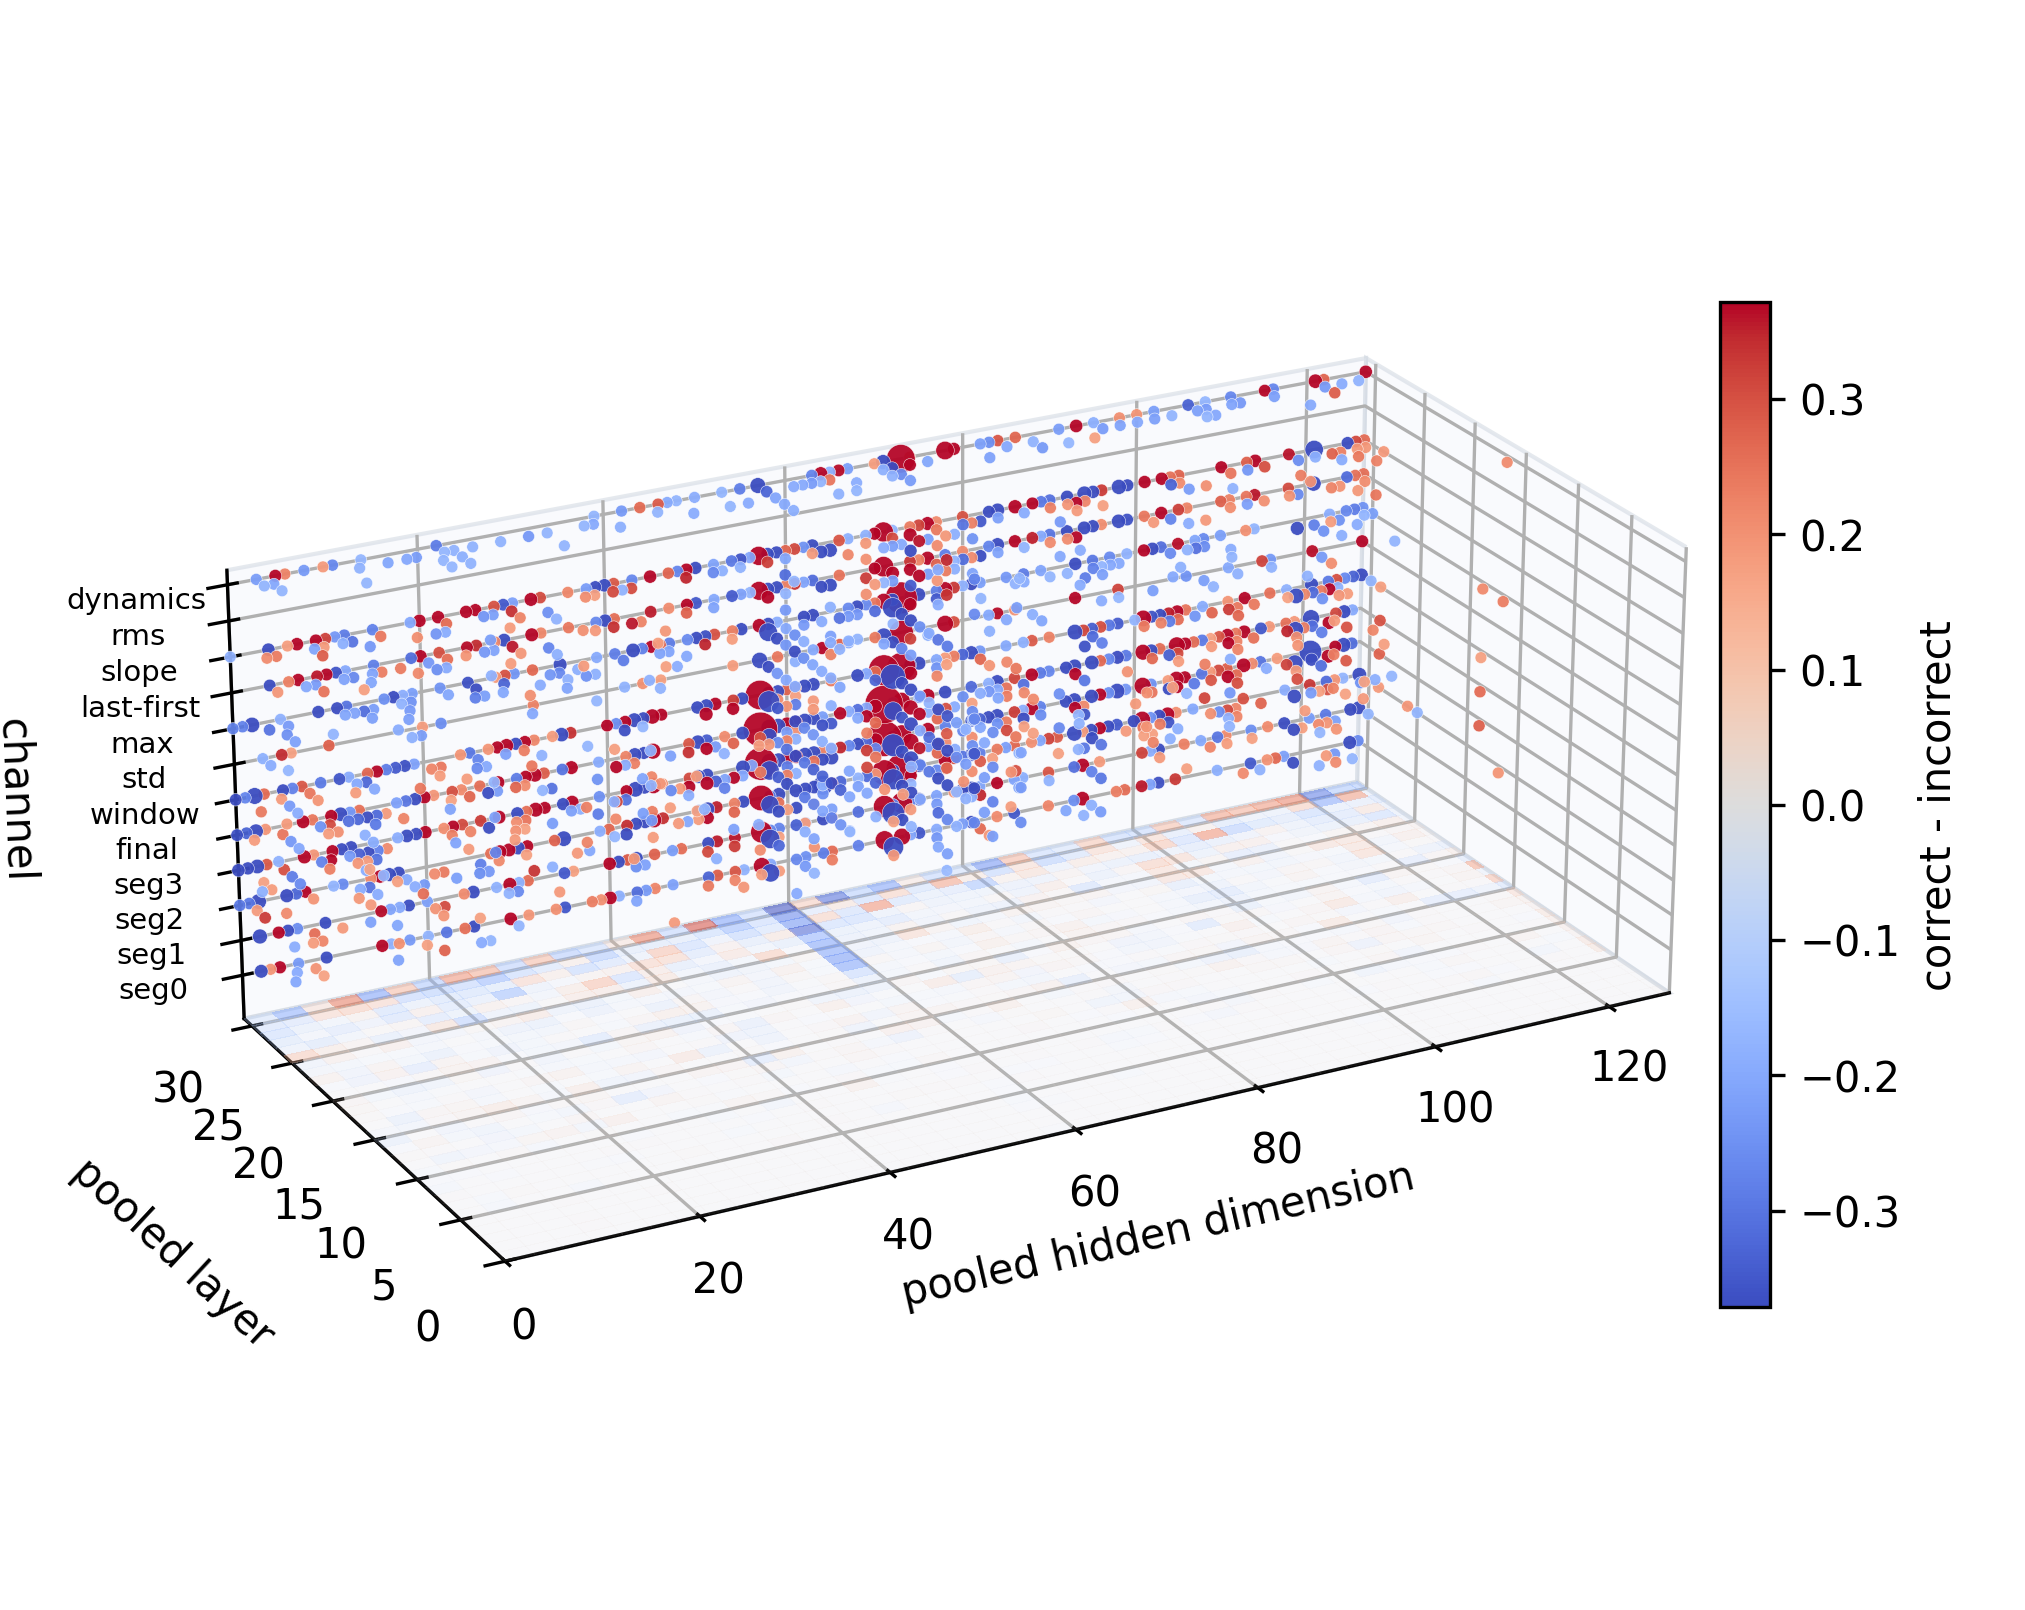
\includegraphics[width=0.88\linewidth]{figures/actmap_volume_signature.png}
    \caption{Mean class-discriminative signature of \actmap{}: the difference between the mean activation map of correct answers and that of incorrect answers, averaged over the TriviaQA training set. Warmer regions, which appear across layers and temporal channels rather than in one layer, mark where the internal state differs most systematically between correct and incorrect generations.}
    \label{fig:actmap}
\end{figure}

\subsection{Classifier}
\label{sec:classifier}

The \actmap{} representation is a three-dimensional tensor, and the classifier must exploit both the layer-depth axis and the temporal-channel axis simultaneously. Several architectures were evaluated on a held-out validation subset before committing to the full three-seed benchmark.

ResNet-style convolutional networks were tested first. They achieved competitive AUROC on TriviaQA but degraded noticeably on NQ-Open, suggesting that local receptive fields miss longer-range structure across the layer axis. A ConvNeXt-small variant performed better, closing most of the NQ-Open gap, but at roughly 28 million parameters it introduced non-trivial inference overhead relative to the feature-extraction cost of the uncertainty signal itself.

The final model is a compact ViT2D classifier trained from scratch on \(12 \times 32 \times 128\) activation maps. The architecture splits each map into non-overlapping \(4 \times 16\) patches, yielding an \(8 \times 8\) grid of 64 tokens, and uses 192-dimensional embeddings, 6 transformer blocks, 6 attention heads, dropout 0.3, attention dropout 0.1, and stochastic depth 0.05. This design has approximately 2.3 million parameters. The classifier is lightweight relative to the 8B LLMs: in optimized batch-one timing on an RTX 5090 Laptop GPU, the ViT forward pass had median latency of about 0.85 ms. Keeping a representative Qwen3-8B hidden-state tensor on GPU, \actmap{} construction added about 0.24 ms, for a combined post-generation median of about 1.20 ms before any serving-specific hook overhead. This places the total post-generation cost well below autoregressive answer generation, though both the map construction and the ViT pass are part of the real online budget and should be accounted for in deployment. The attention mechanism lets the classifier attend globally across both the layer and channel axes, which explains its advantage over convolutional alternatives on out-of-distribution splits. Each seed trains independently with the same split seed used by the corresponding benchmark fold. Results are reported as mean and approximate 95\% confidence interval across seeds 42, 123, and 456.

This classifier should be read as a strong but not fully optimized use of the representation. Preliminary TriviaQA runs suggest that more extensive model selection and ensembling could improve performance: for example, a two-seed ViT2D ensemble reached about 0.886 AUROC on the earlier 30k TriviaQA test split, compared with about 0.879 for the corresponding single ViT2D run. The present study therefore prioritizes introducing and evaluating the \actmap{} representation over exhaustively optimizing the training recipe or deployment stack.

\subsection{Training}

All \actmap{} classifiers share a single training recipe across datasets and seeds. Maps are split by question with grouped shuffling, so no question appears in more than one split and the test score cannot be inflated by near-duplicate phrasings of the same fact. The classifier emits a single logit and is trained with binary cross-entropy. Because the benchmarks are not perfectly balanced, the positive class is reweighted by the empirical negative-to-positive ratio, which prevents the loss from collapsing toward the majority label on skewed datasets such as WebQuestions.

Optimization uses AdamW with learning rate \(10^{-3}\), weight decay \(0.05\), and a cosine schedule with five warmup epochs decaying to a small floor. Training runs for up to 80 epochs with early stopping on validation AUROC (patience 20), and the checkpoint with the best validation AUROC is restored for the final test pass. Two augmentations counter overfitting on the information-dense maps: additive Gaussian noise (standard deviation 0.08) applied to each training map, and mixup with \(\alpha=0.2\), which linearly interpolates pairs of maps and their labels. Gradients are clipped to norm 1.0 and the batch size is 64. Combined with the dropout, attention dropout, and stochastic depth noted above, this recipe is deliberately conservative, because the activation maps are high-dimensional and some training sets, especially NQ-Open, are small.

Spatial position is encoded with factorized row and column embeddings added to each patch, together with a separate learned position for the classification token, whose final representation is read out through a small two-layer GELU head. The factorized encoding respects the asymmetry of the map: its two spatial axes, transformer depth and hidden-dimension bins, are not interchangeable, so they receive independent positional parameters rather than a single shared grid embedding.

\subsection{Baselines}

\textbf{Black-box baselines.} The black-box baselines use only externally available model outputs. They require no hidden states and no supervised training on the \actmap{} labels, but they also see a much narrower view of the generation process. The definitions below describe the exact scoring rules used in this evaluation.

\textbf{Mean token entropy (MTE).} MTE measures how uncertain the LLM is over the answer tokens themselves. For a question \(q\) and generated answer \(a_{1:T}\), let \(p_t(v)=p(v \mid q,a_{<t})\) be the next-token distribution at answer position \(t\). In the implementation, entropy is computed from the logged top-token support \(\mathcal{V}_t\), renormalized as \(\tilde p_t\). The score is
\[
    \mathrm{MTE}(q,a)
    =
    \frac{1}{T}\sum_{t=1}^{T}
    \left(
        -\sum_{v \in \mathcal{V}_t} \tilde p_t(v)\log \tilde p_t(v)
    \right).
\]
High MTE means the model distributed probability mass across many plausible next tokens while producing the answer, so it is naturally an uncertainty score. For AUROC and AUPRC, where larger scores should indicate a more likely correct answer, the reported confidence score is \(s_{\mathrm{MTE}}=-\mathrm{MTE}(q,a)\). To reduce tokenization boundary artifacts, the answer is scored in plain, space-prefixed, and newline-prefixed form, and the variant with the highest mean answer-token log probability is kept.

\textbf{P(True).} \(P(\mathrm{True})\) follows the confidence-elicitation idea that a language model can be asked to judge whether a proposed answer is correct~\cite{kadavath2022}. The model receives a separate scoring prompt containing the question and generated answer, followed by an instruction to respond only with \texttt{True} or \texttt{False}. If \(\pi(q,a)\) denotes this prompt, \(\mathcal{T}\) the single-token variants of \texttt{True}, and \(\mathcal{F}\) the single-token variants of \texttt{False}, the confidence score is
\[
    s_{P(\mathrm{True})}(q,a)
    =
    \frac{\sum_{v \in \mathcal{T}} p(v \mid \pi(q,a))}
    {\sum_{v \in \mathcal{T}} p(v \mid \pi(q,a)) +
     \sum_{v \in \mathcal{F}} p(v \mid \pi(q,a))}.
\]
This baseline therefore measures the model's self-evaluated probability that the proposed answer is correct, normalized over the two allowed verbal labels. It is still black-box because it uses only output-token probabilities, but unlike MTE it requires an additional short forward pass with the self-evaluation prompt.

Semantic sampling and explanation consistency methods were omitted from the benchmark because of their computational cost. Although they are relevant uncertainty estimators, they require multiple generations per question together with clustering, entailment comparisons, or stable explanation checks~\cite{becker2024,farquhar2024}.

\textbf{DRIFT-style MLP.} DRIFT~\cite{bhatnagar2026} is a recent supervised representation-based method for hallucination detection and one of the strongest white-box UQ references. No official source code was available, and the paper's strongest transformer detector is not fully specified at the hyperparameter level, so this report uses a transparent best-effort reproduction: a single consistent DRIFT-style MLP baseline in both the main benchmark and the Qwen2.5 stress test. Unlike \actmap{}, this baseline uses prompt-side prefill features, not generated-token trajectories: hidden states are read at the last question token before \texttt{Answer:}. It uses HuggingFace hidden-state indices \(\{1,5,9,13,17,21\}\), corresponding to transformer layers \(\{0,4,8,12,16,20\}\) because \texttt{hidden\_states[0]} is the embedding output. In the main three-model benchmark this gives a \(24576\)-dimensional concatenated vector. The classifier is a \(24576 \rightarrow 512 \rightarrow 128 \rightarrow 2\) MLP with LeakyReLU, dropout 0.3, cross-entropy loss, AdamW, learning rate \(10^{-4}\), weight decay \(10^{-3}\), batch size 64, patience 8, and standardized features. In the separate Qwen2.5 stress test the same extraction and classifier recipe produce a \(21504\)-dimensional feature vector because Qwen2.5-7B has hidden size 3584.

\textbf{Best-layer linear probe.} This is a deliberately simple white-box baseline. It trains one affine two-logit classifier per hidden layer on the same prompt-side last-question-token features, selects the layer with best source-validation AUROC, and evaluates that selected layer on the target split. This baseline is important because it tests whether \actmap{} gains come from genuine trajectory structure rather than just choosing a good layer.

\section{Experimental Protocol}

The main LLMs are Qwen3-8B~\cite{qwen3}, Llama-3.1-8B-Instruct~\cite{llama3}, and Mistral-7B-Instruct-v0.3~\cite{mistral7b}. All generated answers use greedy decoding. For Qwen3, the chat template is called with \texttt{enable\_thinking=False}; Llama and Mistral do not use a separate thinking-mode flag in this setup. The evaluation code also strips any accidental \texttt{<think>} block before labeling. Labels are answer-correctness labels computed for the generated answers.

The benchmark uses three concise factual QA datasets plus GSM8K math reasoning. TriviaQA~\cite{triviaqa} is the largest source domain and provides broad coverage of factoid questions, making it useful for training a high-capacity uncertainty detector. NQ-Open is derived from Natural Questions~\cite{naturalquestions} and uses natural search-style questions; it tests whether the learned signal transfers to a different question distribution and a smaller balanced benchmark. WebQuestions~\cite{webquestions} is more entity- and relation-centric, originating from question-answer pairs over Freebase, and therefore stresses aliasing and entity matching. GSM8K~\cite{gsm8k} extends the benchmark to grade-school math reasoning. Because GSM8K normally invites step-by-step solutions, the generation prompt asks the model to return only the final numeric answer, without units or explanation. These datasets were chosen because they share the same generated-answer and correctness-label pipeline while differing in size, question style, entity density, reasoning demand, and label balance.

\begin{table}[H]
\centering
\caption{Example source rows before generation. During evaluation, each source question is answered by each LLM and the generated answer is labeled against the reference answer set.}
\footnotesize
\setlength{\tabcolsep}{3pt}
\begin{tabular}{L{2.15cm}L{6.65cm}L{3.55cm}}
\toprule
Dataset & Question & \shortstack[l]{Reference answer\\examples} \\
\midrule
TriviaQA & Which jazz musician and clarinet player was known as the King of Swing? & Benny Goodman \\
NQ-Open & when was the last time anyone was on the moon & 14 December 1972 UTC; December 1972 \\
WebQuestions & what character did john noble play in lord of the rings? & Denethor II \\
GSM8K & Natalia sold clips to 48 of her friends in April, and then she sold half as many in May. How many clips did Natalia sell altogether in April and May? & 72 \\
\bottomrule
\end{tabular}
\label{tab:dataset-examples}
\end{table}

\begin{table}[H]
\centering
\caption{Datasets and split protocol. Splits are grouped by question and repeated for seeds 42, 123, and 456.}
\small
\setlength{\tabcolsep}{4pt}
\begin{tabular}{lrrr@{\,/\,}r@{\,/\,}r}
\toprule
Dataset & Rows & Correct rate & \multicolumn{3}{c}{Train / Val / Test} \\
\midrule
TriviaQA~\cite{triviaqa} & 90,000 & 59.5\% & 72,000 & 9,000 & 9,000 \\
NQ-Open~\cite{naturalquestions} & 4,296 & 50.0\% & 3,431 & 429 & 436 \\
WebQuestions~\cite{webquestions} & 17,430 & 45.1\% & 13,944 & 1,743 & 1,743 \\
GSM8K~\cite{gsm8k} & 9,638 & 50.0\% & 7,688 & 986 & 964 \\
\bottomrule
\end{tabular}
\label{tab:data}
\end{table}



For every source-target pair, a model is trained on the source training split and evaluated on the target test split for the same seed. This gives a \(4 \times 4\) transfer matrix for \actmap{}, DRIFT, and the linear probe. Black-box baselines are evaluated on each dataset's held-out test split and summarized across seeds. Confidence intervals are \(1.96\,s/\sqrt{3}\) across the three seeds, so they should be interpreted as seed variability estimates rather than large-sample uncertainty intervals.

Three metrics are reported throughout. \textbf{AUROC} (Area Under the Receiver Operating Characteristic curve) measures ranking quality: the probability that a randomly chosen correct answer receives a higher confidence score than a randomly chosen incorrect one, with 0.5 being chance and 1.0 being perfect. \textbf{AUPRC} (Area Under the Precision-Recall Curve) captures the trade-off between precision and recall across all score thresholds and is more informative than AUROC under class imbalance. \textbf{ECE} (Expected Calibration Error) measures the average gap between predicted confidence and observed accuracy; lower is better, with 0 indicating a perfectly calibrated model.

\section{Results}

\subsection{In-Domain Benchmark}

\begin{figure}[H]
    \centering
    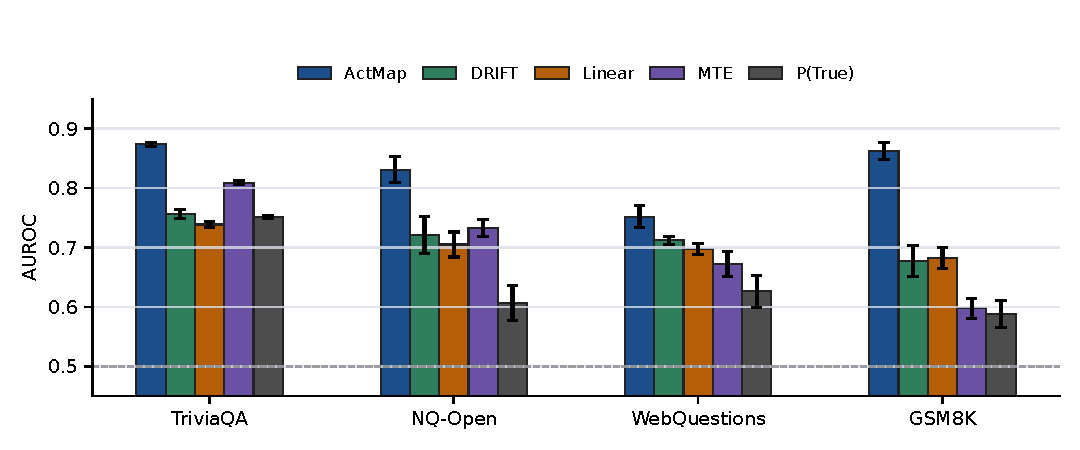
\includegraphics[width=0.88\linewidth]{figures/final/indomain_auroc_comparison.pdf}
    \caption{In-domain AUROC on the three factual QA datasets and GSM8K, with 95\% confidence intervals across three seeds. \actmap{} attains the highest mean AUROC in every benchmark group.}
    \label{fig:indomain}
\end{figure}

\begin{table}[H]
\centering
\caption{In-domain AUROC, mean \(\ci\) 95\% CI across seeds. Bold marks the best method per dataset.}
\footnotesize
\setlength{\tabcolsep}{3pt}
\begin{tabular}{lccccc}
\toprule
Dataset & \actmap{} & DRIFT & Linear & MTE & \(P(\mathrm{True})\) \\
\midrule
TriviaQA & \textbf{0.873 \(\ci\) 0.003} & 0.756 \(\ci\) 0.008 & 0.739 \(\ci\) 0.006 & 0.809 \(\ci\) 0.004 & 0.752 \(\ci\) 0.003 \\
NQ-Open & \textbf{0.831 \(\ci\) 0.022} & 0.720 \(\ci\) 0.031 & 0.705 \(\ci\) 0.021 & 0.732 \(\ci\) 0.014 & 0.607 \(\ci\) 0.029 \\
WebQuestions & \textbf{0.752 \(\ci\) 0.018} & 0.712 \(\ci\) 0.007 & 0.697 \(\ci\) 0.010 & 0.672 \(\ci\) 0.021 & 0.626 \(\ci\) 0.027 \\
GSM8K & \textbf{0.863 \(\ci\) 0.014} & 0.677 \(\ci\) 0.026 & 0.682 \(\ci\) 0.018 & 0.598 \(\ci\) 0.017 & 0.588 \(\ci\) 0.022 \\
\bottomrule
\end{tabular}
\label{tab:indomain}
\end{table}

Ranking quality is measured in-domain, with each detector trained and tested on the same benchmark. The margin over the next-best method is largest on TriviaQA, where \actmap{} beats DRIFT by \(+0.117\) AUROC and the strongest black-box baseline by \(+0.064\). On NQ-Open, \actmap{} beats the strongest retained black-box baseline by \(+0.098\) AUROC and DRIFT by \(+0.110\). WebQuestions is harder, but \actmap{} still leads DRIFT by \(+0.040\), the linear probe by \(+0.055\), and MTE by \(+0.079\). GSM8K shows the signal extends beyond factoid entity QA: on numeric math answers \actmap{} leads DRIFT by \(+0.185\), the linear probe by \(+0.181\), and MTE by \(+0.265\).

\subsection{Transferability}

\begin{figure}[H]
    \centering
    \makebox[\linewidth][c]{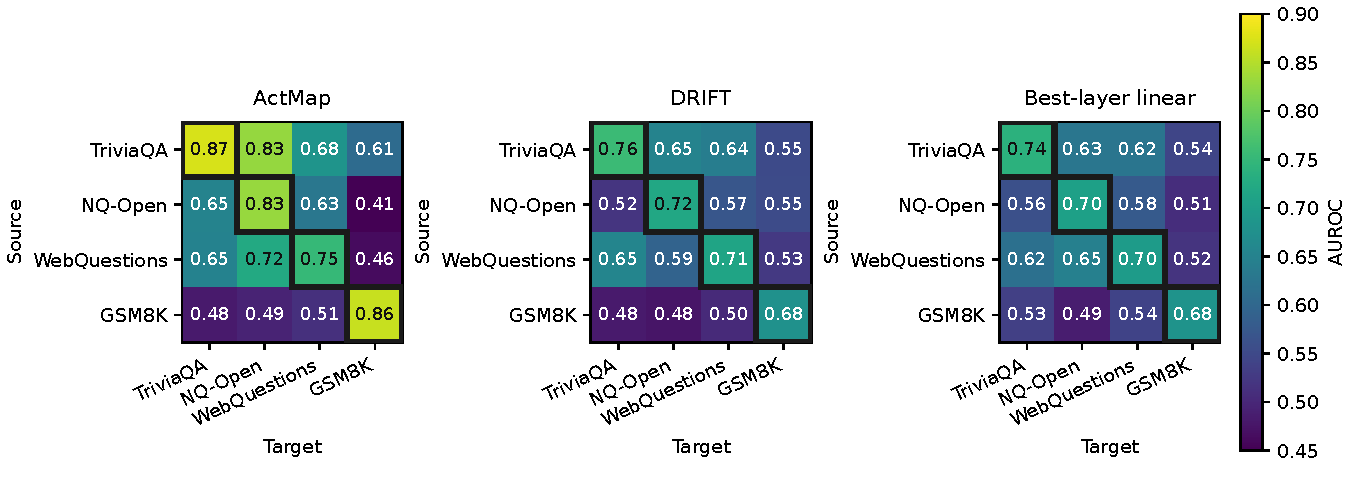
\includegraphics[width=1.12\linewidth]{figures/final/transfer_auroc_matrices.pdf}}
    \caption{Source-to-target AUROC matrices for \actmap{}, DRIFT, and the best-layer linear probe. Rows are training datasets and columns are evaluation datasets. Each cell is the mean AUROC across three seeds.}
    \label{fig:transfer}
\end{figure}

Distribution shift tests whether a correctness detector trained on one question distribution still ranks answers correctly on another distribution without target-domain tuning. In-domain evaluation can instead reward dataset-specific shortcuts: a classifier trained and tested on the same benchmark may learn answer-length, prompt-style, or LLM-specific regularities that do not reflect a general uncertainty signal. This is the setting needed for routing or abstention systems that will see new question mixtures after deployment.

Transfer is asymmetric. \actmap{} trained on TriviaQA transfers strongly to NQ-Open, almost matching the NQ-Open in-domain result (\(0.831 \ci 0.022\)), whereas the reverse direction is much weaker. The most plausible explanation is source coverage. TriviaQA supplies a much larger and more varied factoid training distribution, so it exposes the classifier to a broader set of correct and incorrect generation trajectories. NQ-Open is smaller in this benchmark, so its learned boundary transfers less effectively to the broader TriviaQA test set.

\actmap{} works best when the source and target share short-answer factual QA structure: TriviaQA-to-NQ-Open is the clearest case, and WebQuestions-to-NQ-Open remains useful. Transfer into WebQuestions is harder in both directions. WebQuestions is more entity- and relation-centric, has a lower correct-answer rate, and is more sensitive to aliasing, so the source-domain decision boundary does not carry over as cleanly.

\actmap{} is more robust than the single-token white-box baselines under factual QA shifts because it does not rely on one prompt-position hidden state. It observes the full answer trajectory through segment means, final-token state, late-window state, temporal slope, and token dynamics, then lets the ViT attend globally across channels and layers. This gives the classifier multiple chances to detect hesitation, late correction, or unstable generation patterns that survive a dataset change. The advantage over DRIFT is largest on TriviaQA-to-NQ-Open (\(+0.178\) AUROC) and WebQuestions-to-NQ-Open (\(+0.130\)). The exception is WebQuestions-to-TriviaQA, where \actmap{} and DRIFT are effectively tied, again indicating that WebQuestions is a narrower source domain for the broader TriviaQA target.

GSM8K changes the transfer picture. \actmap{} remains strong on GSM8K in-domain, but factual-QA checkpoints do not transfer reliably into math reasoning, and the weakest pairings fall below chance. The reverse direction, from GSM8K into factual QA, is also narrow. \actmap{} therefore detects a real correctness signal in reasoning-style numeric answers, but the learned boundary is domain-specific unless the source data covers the target answer regime.

\subsection{Mixed-Source Transfer}

Source coverage is evaluated directly with balanced mixed-source \actmap{} probes, which separate whether the GSM8K transfer gap reflects limited source coverage or an unusable representation. Each mixed training set is balanced per source dataset, LLM, and correctness label, then evaluated on the original target test splits.

\begin{table}[H]
\centering
\caption{Mixed-source \actmap{} transfer, mean target-test AUROC \(\ci\) 95\% CI across three seeds. WebQ abbreviates WebQuestions; a dash marks a target not evaluated for that training mixture.}
\small
\setlength{\tabcolsep}{5pt}
\begin{tabular}{L{3.2cm}cccc}
\toprule
Training sources & TriviaQA & NQ-Open & WebQuestions & GSM8K \\
\midrule
TriviaQA + GSM8K & \(0.713 \ci 0.024\) & -- & -- & \textbf{0.829} \(\ci\) \textbf{0.013} \\
NQ-Open + GSM8K & -- & \textbf{0.828} \(\ci\) \textbf{0.038} & -- & \(0.813 \ci 0.014\) \\
WebQ + GSM8K & -- & -- & \(0.647 \ci 0.017\) & \textbf{0.829} \(\ci\) \textbf{0.016} \\
All QA datasets & \textbf{0.715} \(\ci\) \textbf{0.015} & \(0.804 \ci 0.029\) & \textbf{0.680} \(\ci\) \textbf{0.010} & \(0.524 \ci 0.073\) \\
All four datasets & \(0.711 \ci 0.023\) & \(0.791 \ci 0.010\) & \(0.668 \ci 0.023\) & \(0.826 \ci 0.031\) \\
\bottomrule
\end{tabular}
\label{tab:mixed-source}
\end{table}

Mixed-source training supports the source-coverage interpretation while complicating the usual ``more data is always better'' story. Adding GSM8K to each factual-QA source raises GSM8K transfer far above single-source factual-QA transfer, while the factual-QA-only mixture still leaves GSM8K near chance, confirming that math/reasoning examples are needed. Mixed probes also trade away target-specific QA performance: the all-four source recovers GSM8K but stays below the in-domain models on TriviaQA and WebQuestions. Source coverage therefore reduces the reasoning-domain transfer gap, while target-domain validation remains important when maximum in-domain ranking performance matters.

To investigate whether the mixed-source performance drop stems from a model capacity bottleneck, we evaluated a larger ``ViT2D-Medium'' variant (18.1M parameters, embedding dimension 384, 12 layers) trained on the all-four dataset mixture. The larger architecture failed to recover the performance gap and further degraded mean AUROC to \(0.663\) on TriviaQA and \(0.636\) on WebQuestions, compared to the \(0.711\) and \(0.668\) achieved by our compact 2.3M-parameter Small baseline. This decline rules out insufficient model capacity as the limiting factor. Instead, it suggests a phenomenon of negative transfer or multi-task optimization interference, where capturing the distinct activation geometry of math reasoning fundamentally conflicts with or alters the representations needed to rank factual QA trajectories.

\begin{table}[H]
\centering
\caption{Capacity sweep on the four-source mixture: scaling the \actmap{} ViT2D classifier degrades target performance, confirming multi-task interference over a parameter bottleneck. Mean target-test AUROC.}
\small
\setlength{\tabcolsep}{6pt}
\begin{tabular}{L{3.2cm}ccc}
\toprule
Target split & In-Domain Small ViT & All-Four Small ViT & All-Four Medium ViT \\
\midrule
TriviaQA & 0.873 & \(0.711\) & \(0.663\) \\
WebQuestions & 0.752 & \(0.668\) & \(0.636\) \\
\bottomrule
\end{tabular}
\label{tab:capacity-sweep}
\end{table}

\subsection{Qwen2.5 DRIFT-Style Stress Test}

Stress-test reproducibility is evaluated in the model and dataset setting the DRIFT paper emphasizes: \texttt{Qwen/Qwen2.5-7B-Instruct}~\cite{qwen25} with standard TriviaQA validation, where DRIFT reports \(0.9395\) AUROC for its strongest setting. Kept separate to avoid mixing protocols, this stress test applies Qwen2.5-7B to 17,944 TriviaQA validation questions with the prompt \texttt{Question: \{q\}\textbackslash{}nAnswer:} and greedy decoding. The \actmap{} row uses the generated-token decoding trajectory. The DRIFT row is the prompt-prefill reproduction: six last-question-token hidden states before \texttt{Answer:}.

\begin{table}[H]
\centering
\caption{Qwen2.5-7B-Instruct stress test on TriviaQA validation (single seed). \actmap{} uses the generated-token decoding trajectory; DRIFT uses prompt-prefill last-question-token features. Bold marks the better result per column.}
\begin{tabular}{lrrrr}
\toprule
Method & Test rows & AUROC & AUPRC & ECE \\
\midrule
\actmap{} (ViT2D) & 3,590 & \textbf{0.9444} & 0.8926 & \textbf{0.0288} \\
DRIFT & 3,590 & 0.9328 & \textbf{0.8945} & 0.0811 \\
\bottomrule
\end{tabular}
\label{tab:qwen25}
\end{table}

The reproduced DRIFT-style baseline lands close to the paper's reported \(0.9395\) AUROC, which supports that the implementation captures the intended signal in the original high-performing setting. This matters for the main benchmark: DRIFT's weaker NQ-Open result is unlikely to reflect a failed reproduction. DRIFT is instead highly sensitive to model, dataset, and protocol choices; Qwen2.5 on TriviaQA is a favorable setting, while the same baseline generalizes much less strongly to the three-model NQ-Open benchmark. \actmap{} nonetheless leads on AUROC in the stress test and substantially improves calibration, cutting ECE to roughly a third of DRIFT's, so its confidence scores align much better with empirical accuracy for deployment decisions such as abstention thresholds.

\subsection{Ablations and Calibration}

The channel ablation tests the central design claim: that the full generation trajectory carries more correctness signal than any single temporal statistic. On a held-out source subset, masking all channels collapses performance to chance, confirming that the signal comes from activation content rather than label leakage in the pipeline. Keeping only early-segment information is much weaker: at the start of generation the answer is not yet committed, so early activations are less diagnostic of final correctness. The final-token and late-segment channels are the strongest single predictors, consistent with the answer being most fully represented once produced. The dynamics channels (temporal slope, absolute step-to-step change, and the last-minus-first difference) are weaker in isolation but improve robustness when combined with the rest of the map, capturing hesitation or late-correction patterns that the static summaries miss. This also explains why \actmap{} outperforms the best-layer linear probe, which reads only one prompt-position hidden state and cannot observe this temporal structure.

\begin{figure}[H]
    \centering
    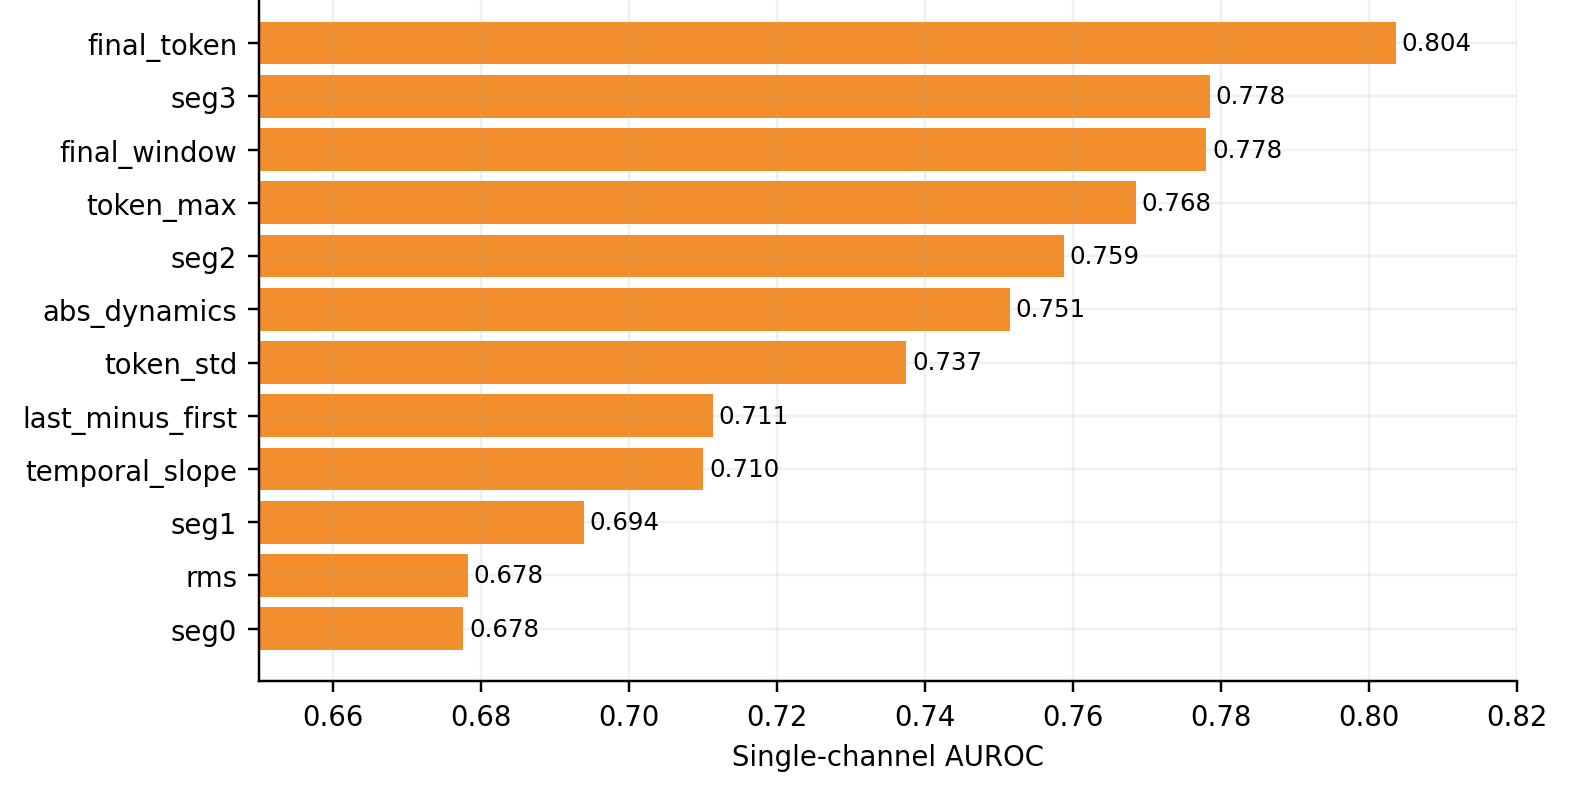
\includegraphics[width=0.67\linewidth]{figures/channel_ablation.png}
    \caption{Channel ablation on a held-out source subset. Each bar reports AUROC for a representation that keeps or masks a subset of the twelve \actmap{} channels.}
    \label{fig:ablation}
\end{figure}

Calibration is mixed. On TriviaQA, \actmap{} has low ECE (\(0.026 \ci 0.013\)), comparable to DRIFT and the linear probe. On GSM8K, ECE is also moderate (\(0.059 \ci 0.024\)). On NQ-Open, \actmap{} remains the best ranker but its ECE rises to \(0.093 \ci 0.071\). On WebQuestions, \actmap{} again has the best AUROC but ECE is \(0.102 \ci 0.021\), worse than DRIFT and the linear probe. For deployment, \actmap{} should therefore be treated primarily as a ranking and routing signal unless calibrated on target-domain validation data.

\section{Fairness, Latency, and Reproducibility}

\begin{table}[H]
\centering
\caption{Fairness and latency comparison. Online cost excludes the base autoregressive answer generation shared by all methods that need an answer.}
\small
\setlength{\tabcolsep}{4pt}
\begin{tabular}{L{1.7cm}L{3.0cm}L{2.6cm}L{4.25cm}}
\toprule
Method & Input signal & Extra model pass & Online cost after answer generation \\
\midrule
\actmap{} & Generated-token hidden-state trajectory & no separate prompt pass & GPU map build + ViT: \(\sim\)1.2 ms median; hook cost depends on serving setup \\
DRIFT & six prompt-side hidden states & no if captured during prefill; otherwise yes & lightweight MLP after hidden-state extraction \\
Linear & one prompt-side hidden state & no if captured during prefill; otherwise yes & cheapest white-box classifier after feature extraction \\
MTE & answer-token probabilities & no if logprobs are already returned & cheap when serving engine exposes token logprobs \\
\(P(\mathrm{True})\) & model self-evaluation prompt & yes & one additional short scoring prompt \\
\bottomrule
\end{tabular}
\label{tab:fairness}
\end{table}

The protocol matters for fairness. The same splits are used across methods. White baselines train once per source dataset and seed, then evaluate all targets. Black baselines score each held-out row once and reuse those scores for all seed summaries. The figures are generated from aggregated experiment summaries rather than hand-entered numbers. Post-generation latency figures are reported in Section~\ref{sec:classifier} and exclude base decoding and any serving-specific hook overhead.

\section{Interpretability and Ethical Implications}

\actmap{} should be read as an operational interpretability artifact rather than a natural-language explanation. Its value is modest but useful: it creates a stable intermediate artifact tied to each generated answer. That artifact has meaningful axes: transformer depth, hidden-dimension bins, and temporal channels over the answer trajectory. This makes it possible to inspect aggregate class signatures, run channel ablations, compare LLM-specific behavior, and monitor distribution shift. The method therefore sits between opaque scalar confidence and full mechanistic explanation.

This is ethically favorable in several ways. First, it can support \textbf{human oversight}. A system can route low-confidence answers to a human, retrieval pipeline, or stronger model rather than silently returning a fluent guess. Second, it can reduce \textbf{overreliance}. Users tend to trust confident language; an uncertainty score gives the interface a technical basis for warnings or abstention. Third, it improves \textbf{accountability}. If a deployed model fails, logged uncertainty scores and activation-map summaries can help determine whether the system had evidence of risk before returning the answer. Fourth, it supports \textbf{proportionality}. Expensive verification does not need to run on every query; it can be allocated to the examples most likely to be wrong.

The work is also favorable from an interpretability-governance perspective. The NLA article shows one route toward making activations legible through natural language. \actmap{} follows the same broad intuition that activations are worth auditing, while choosing a narrower measurable target: answer correctness. This makes the method easier to validate quantitatively. The resulting map is a reusable object for technical oversight. A regulator or internal safety team can ask concrete questions: Does the model's uncertainty degrade on a new dataset? Does one LLM family show systematically different activation signatures? Are late-token dynamics more predictive than early-token summaries? Do calibration errors concentrate on a specific benchmark?

There are still risks. Hidden states may encode information about prompts or generated content, so activation logs should be minimized, access-controlled, and deleted or aggregated when possible. A risk score can also be misused as a veneer of safety if it is shown without calibration evidence. The correct deployment posture is therefore conservative: use \actmap{} to trigger review, abstention, or additional verification rather than to certify that an answer is true. Under that posture, the ethical implications are mostly positive: the method gives systems a way to recognize and expose uncertainty instead of hiding it behind fluent text.

\section{Limitations}

\begin{itemize}
    \item \textbf{Scope.} The benchmark is short-answer QA plus GSM8K-style numeric reasoning. Longer free-form reasoning, dialogue, summarization, and tool-use tasks may require different activation summaries.
    \item \textbf{White-box access.} \actmap{}, DRIFT, and the linear probe require hidden states. They are not available for ordinary closed APIs unless providers expose trusted activation features.
    \item \textbf{Answer labels.} Labels are benchmark-match labels for concise generated answers: aliases for factual QA and numeric matching for GSM8K. Alias coverage and normalization matter, especially for WebQuestions-style entity answers.
    \item \textbf{Calibration.} Ranking performance is strong across the evaluated QA datasets, but calibrated probabilities do not transfer automatically. Target-domain recalibration is needed.
    \item \textbf{Causality.} \actmap{} detects correlates of correctness; it does not prove why the model knows or fails.
\end{itemize}

\section{Next Steps}

GSM8K partially addresses benchmark breadth by adding reasoning-style numeric answers, but the transfer and mixed-source results show that source coverage remains a central open problem. Balanced mixed-source training reduces the QA-to-math gap, but it does not yet preserve the best target-specific AUROC on every dataset. A broader comparison against additional state-of-the-art uncertainty methods, covering semantic sampling, explanation-consistency probes, and ensemble-based estimators, is also needed; this was not conducted in the present work due to time constraints.

The first next step is to adapt the \actmap{} idea to uncertainty quantification for graph models. A Graph-ActMap version would record GNN or GAT message-passing trajectories as fixed tensors over layers, ego/one-hop/two-hop neighborhoods, hidden-feature bins, and attention-routing statistics, then train a small probe to detect misclassified or out-of-distribution graph predictions from that local computation footprint. This would test whether reliability is visible not only in LLM token trajectories, but also in how graph evidence is aggregated, smoothed, or routed through neighborhoods.

The second next step is systems-oriented. \actmap{} is naturally suited to adaptive retrieval-augmented generation: a model can answer directly when the uncertainty signal is low-risk and trigger retrieval only when the activation trajectory suggests a likely failure. This would use uncertainty to spend retrieval and verification budget where it is most useful.

The third next step is learning-oriented. If \actmap{} captures a robust uncertainty signal, it could become a reward, penalty, or auxiliary objective in reinforcement learning. A policy could be rewarded for trajectories that look internally stable and penalized for confident-looking text produced from high-uncertainty activation dynamics.

Calibration remains necessary for all three directions. The current evidence is strongest for ranking and routing, but real deployments need reliable probability thresholds. Temperature scaling, isotonic regression, and conformal abstention should be evaluated on held-out target-domain validation sets.

\section{Conclusion}

\actmap{} turns runtime hidden-state trajectories into an image-like uncertainty signal. Across three seeds, it is the strongest in-domain method on TriviaQA, NQ-Open, WebQuestions, and GSM8K; it also beats DRIFT on the best-effort Qwen2.5 DRIFT reproduction in AUROC and calibration. Transfer remains uneven: factual QA sources transfer best to other factual QA targets, while GSM8K exposes a sharper reasoning-domain boundary. The main claim is nonetheless stronger after adding GSM8K because \actmap{} remains ahead of supervised white-box probes and black-box confidence scores under a fourth answer regime.

The central result is both technical and practical. \actmap{} improves AUROC while producing a reusable audit artifact tied to each generated answer. If language models are deployed in settings where fluent wrong answers matter, systems should expose uncertainty, support oversight, and leave inspectable evidence. \actmap{} is a step in that direction.

\begingroup
\footnotesize
\begin{thebibliography}{20}
\raggedright
\setlength{\itemsep}{0pt}
\setlength{\parsep}{0pt}
\setlength{\parskip}{0pt}

\bibitem{azaria2023}
A. Azaria and T. Mitchell.
\newblock The Internal State of an LLM Knows When It's Lying.
\newblock arXiv:2304.13734, 2023.

\bibitem{becker2024}
E. Becker and S. Soatto.
\newblock Cycles of Thought: Measuring LLM Confidence through Stable Explanations.
\newblock arXiv:2406.03441, 2024.

\bibitem{webquestions}
J. Berant, A. Chou, R. Frostig, and P. Liang.
\newblock Semantic Parsing on Freebase from Question-Answer Pairs.
\newblock EMNLP, 2013.

\bibitem{bhatnagar2026}
R. Bhatnagar, Y. Sun, C. A. Zhang, Y. Wen, and H. Yang.
\newblock DRIFT: Detecting Representational Inconsistencies for Factual Truthfulness.
\newblock arXiv:2601.14210v2, 2026.

\bibitem{gsm8k}
K. Cobbe, V. Kosaraju, M. Bavarian, M. Chen, H. Jun, L. Kaiser, M. Plappert, J. Tworek, J. Hilton, R. Nakano, C. Hesse, and J. Schulman.
\newblock Training Verifiers to Solve Math Word Problems.
\newblock arXiv:2110.14168, 2021.

\bibitem{farquhar2024}
S. Farquhar, J. Kossen, L. Kuhn, and Y. Gal.
\newblock Detecting hallucinations in large language models using semantic entropy.
\newblock Nature, 2024.

\bibitem{nla2026}
K. Fraser-Taliente, S. Kantamneni, E. Ong, D. Mossing, C. Lu, P. C. Bogdan, E. Ameisen, J. Chen, D. Kishylau, A. Pearce, J. Tarng, A. Wu, J. Wu, Y. Zhang, D. M. Ziegler, E. Hubinger, J. Batson, J. Lindsey, S. Zimmerman, and S. Marks.
\newblock Natural Language Autoencoders Produce Unsupervised Explanations of LLM Activations.
\newblock Anthropic Transformer Circuits Thread, May 7, 2026.
\newblock \url{https://transformer-circuits.pub/2026/nla/index.html\#pastlensinitialized-activation-oracle-regressions}

\bibitem{llama3}
A. Grattafiori et al.
\newblock The Llama 3 Herd of Models.
\newblock arXiv:2407.21783, 2024.

\bibitem{hleg2019}
High-Level Expert Group on Artificial Intelligence.
\newblock Ethics Guidelines for Trustworthy AI.
\newblock European Commission, 2019.

\bibitem{mistral7b}
A. Q. Jiang et al.
\newblock Mistral 7B.
\newblock arXiv:2310.06825, 2023.

\bibitem{triviaqa}
M. Joshi, E. Choi, D. Weld, and L. Zettlemoyer.
\newblock TriviaQA: A Large Scale Distantly Supervised Challenge Dataset for Reading Comprehension.
\newblock ACL, 2017.

\bibitem{kadavath2022}
S. Kadavath et al.
\newblock Language Models (Mostly) Know What They Know.
\newblock arXiv:2207.05221, 2022.

\bibitem{naturalquestions}
T. Kwiatkowski et al.
\newblock Natural Questions: A Benchmark for Question Answering Research.
\newblock TACL, 2019.

\bibitem{mahaut2024}
M. Mahaut, L. Aina, P. Czarnowska, M. Hardalov, T. Muller, and L. Marquez.
\newblock Factual Confidence of LLMs: on Reliability and Robustness of Current Estimators.
\newblock ACL, 2024.

\bibitem{marks2023}
S. Marks and M. Tegmark.
\newblock The Geometry of Truth: Emergent Linear Structure in Large Language Model Representations of True/False Datasets.
\newblock arXiv:2310.06824, 2023.

\bibitem{nist2023}
National Institute of Standards and Technology.
\newblock Artificial Intelligence Risk Management Framework (AI RMF 1.0).
\newblock NIST AI 100-1, 2023.

\bibitem{qwen25}
Qwen Team.
\newblock Qwen2.5 Technical Report.
\newblock arXiv:2412.15115, 2024.

\bibitem{weidinger2021}
L. Weidinger et al.
\newblock Ethical and social risks of harm from Language Models.
\newblock arXiv:2112.04359, 2021.

\bibitem{xiong2024}
M. Xiong, Z. Hu, X. Lu, Y. Li, J. Fu, J. He, and B. Hooi.
\newblock Can LLMs Express Their Uncertainty? An Empirical Evaluation of Confidence Elicitation in LLMs.
\newblock ICLR, 2024.

\bibitem{qwen3}
A. Yang et al.
\newblock Qwen3 Technical Report.
\newblock arXiv:2505.09388, 2025.

\end{thebibliography}
\endgroup

\end{document}
